\documentclass[twocolumn]{myarticle}

\usepackage{mymacros}
\usepackage{parskip}
\usepackage{hyperref}
\usepackage{listings}
\usepackage{booktabs}

\lstset{%
basicstyle=\small\ttfamily,
columns=flexible,
breaklines=true,
numbers=left,
stepnumber=1,}

\newcommand{\mat}[1]{\begin{bmatrix}#1\end{bmatrix}}

\begin{document}

\title{Monte Carlo methods in computational physics}
\author{Casey Daniel and Chris Deimert}
\date{\today}

\maketitle

\section{Introduction}
\label{sec:introduction}

In this report, we explore a number of Monte Carlo numerical methods.
Monte Carlo methods use pseudorandom numbers to explore complicated systems.
These methods tend to converge slowly for simple problems, but can be very efficient for complex problems: especially those with a large number of variables.

\section{Pseudo random numbers}
\label{sec:pseudo_random_numbers}

Monte Carlo methods typically rely heavily on our ability to generate a large quantity of random numbers.
We cannot, of course, generate truly random numbers on a deterministic computer, so we have to approximate them with pseudo-random numbers (PRN's).
Having a reliable PRN generator is thus a key prerequisite to any Monte Carlo method.
In this section, we will study the linear congruential method (LCM) for generating PRN's.
The LCM generates a sequence of pseudo-random integers with the $ n $th integer given by
\begin{align}
    I_{n} &= \left( A I_n + C \right) \! \! \! \! \! \mod M
\end{align}
($ I_0 $ is called the "seed".)
We can then generate a sequence $ x_n = I_n/M $ of pseudo-random real numbers with $ 0 < x_n < 1 $.

A Fortran 90 module was created to implement the LCM generator and can be seen in Section~\ref{subsec:pseudo_random_numbers_module}.
This code was tested in a number of ways, the code for which is in Section~\ref{subsec:pseudo_random_numbers_main_code} and Section~\ref{subsec:pseudo_random_numbers_plotting_code}.)

The first, simplest test used $ I_0 = 3 $, $ A = 7 $, $ C = 0 $, and $ M = 10 $.
The result is a repeating sequence of numbers:
\begin{align}
    x &= 0.1, 0.7, 0.9, 0.3, 0.1, 0.7, 0.9, 0.3, \ldots
\end{align}
This sequence repeats after only 4 numbers, demonstrating why small values of $ M $ are a poor choice.
The sequence will repeat after at most $ M $ numbers, so we must select a high value of $ M $ in order to obtain a long sequence (though high values of $ M $ do not \emph{guarantee} a long sequence).

One useful way to test a pseudo-random number generator is to look at the correlation between each generated number and the number that preceded it.
These can be plotted in a 2D scatter plot: patterns on the scatter plot imply that the pseudo-random number generator is actually predictable and thus not very random.
The correlation plots for three different sets of coefficients are shown in Figures \ref{fig:lcm_test_1}, \ref{fig:lcm_test_2}, and \ref{fig:lcm_test_3}.
Note that a seed of $ I_0 = 1 $ was used in each case.
It is found that the third combination of coefficients provides the best pseudo-random number generator.

\begin{figure}[ht!]
    \begin{center}
    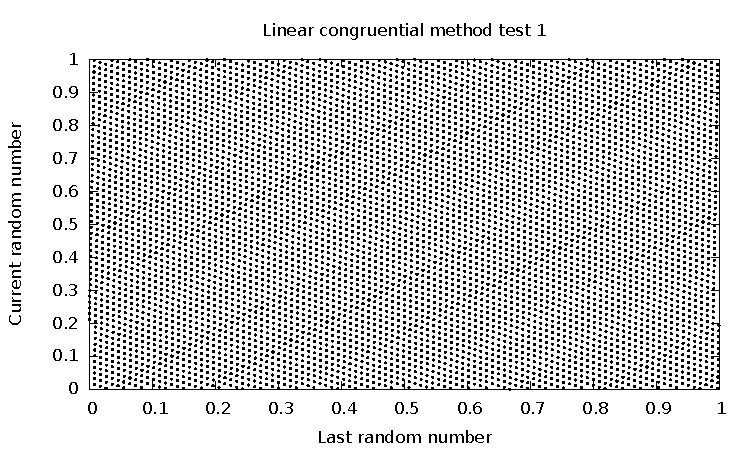
\includegraphics[width = 0.45\textwidth]{../Plots/LCM_test_1.pdf}
    \caption{%
        The correlation plot for $ A = 106 $, $ C = 1283 $, and $ M = 6075 $.
        It is seen that the correlation plot is strongly patterned, meaning that this is a relatively predictable sequence of numbers.
        Thus, this choice of LCM coefficients is a poor one.
    }
    \label{fig:lcm_test_1}
    \end{center}
\end{figure}

\begin{figure}[ht!]
    \begin{center}
    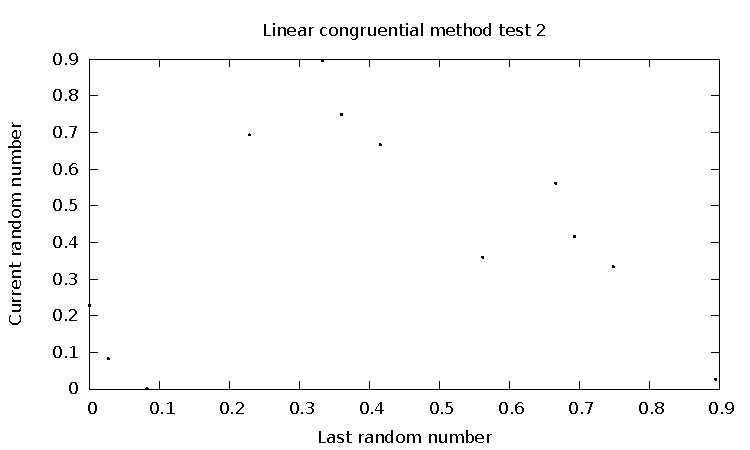
\includegraphics[width = 0.45\textwidth]{../Plots/LCM_test_2.pdf}
    \caption{%
        The correlation plot for $ A = 107 $, $ C = 1283 $, and $ M = 6075 $.
        It is seen that the correlation plot is even more strongly patterned than the last one.
        Thus, this is a relatively predictable sequence of numbers and this choice of LCM coefficients is poor.
        This also demonstrates how small changes in the coefficients lead to drastic changes in the effectiveness of the LCM generator.
        (The coefficients here are the same as the last set except that $ A $ has been increased by 1).
    }
    \label{fig:lcm_test_2}
    \end{center}
\end{figure}

\begin{figure}[ht!]
    \begin{center}
    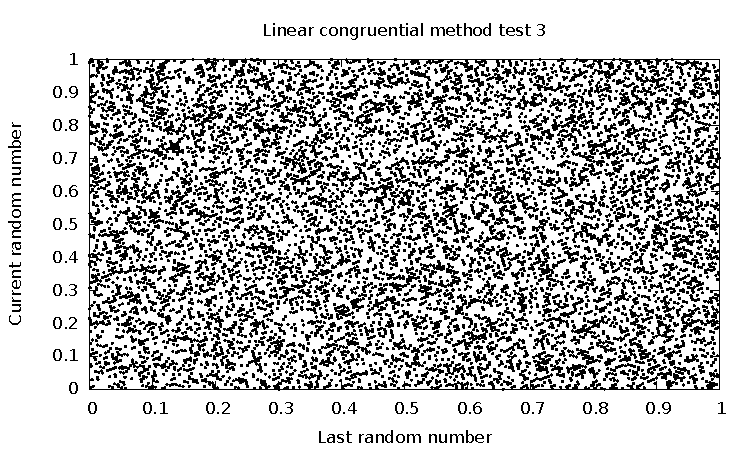
\includegraphics[width = 0.45\textwidth]{../Plots/LCM_test_3.pdf}
    \caption{%
        The correlation plot for $ A = 1103515245 $, $ C = 12345 $, and $ M = 32768 $.
        It is seen that the correlation plot is very weakly patterned, meaning that this is a relatively unpredictable sequence of numbers.
        Thus, this choice of LCM coefficients is a good one.
    }
    \label{fig:lcm_test_3}
    \end{center}
\end{figure}

Another test of pseudo-random number generators that can be performed is a $ \chi^2 $ test.
This is used to determine our statistical confidence in the fact that the pseudo-random numbers are evenly generated.

Using the LCM generator with a seed of $ I_0 = 1 $ and coefficients from the third test above, 100 numbers were generated.
Similarly, 100 numbers were generated using the gfortran generator with a seed based on the computer time.
The distribution of results are shown below.

\bigskip
\begin{center}
    \begin{tabular}{ccccc}
        \toprule
        Interval & Upper limit & LCM & gfortran & Exp. \\
        \midrule
        1  & 0.1 &  6 &  6 & 10 \\
        2  & 0.2 & 11 & 16 & 10 \\
        3  & 0.3 & 12 &  9 & 10 \\
        4  & 0.4 &  9 &  6 & 10 \\
        5  & 0.5 & 10 & 11 & 10 \\
        6  & 0.6 &  9 &  5 & 10 \\
        7  & 0.7 &  8 & 12 & 10 \\
        8  & 0.8 & 10 &  9 & 10 \\
        9  & 0.9 & 11 & 13 & 10 \\
        10 & 1.0 & 14 & 13 & 10 \\
        \bottomrule
    \end{tabular}
\end{center}
\bigskip

The $ \chi^2 $ values for the LCM and gfortran generators are:
\begin{align}
    \chi_{\text{LCM}}^2 &= 6.80
    \\
    \chi_{\text{gfortran}}^2 &= 8.40
\end{align}

These were calculated using 
\begin{align}
    \chi^2 &= \sum_{i=1}^{10} \frac{(O_i - E_i)^2}{E_i}
\end{align}
where $ O_i $ is the observed value in the $ i $th row of the table above, and $ E_i $ is the expeced value. 

It should be noted that the $ \chi^2 $ values change significantly depending on the seed used, though the ones given here are fairly typical.
The LCM $ \chi^2 $ varies from about 2 to about 10, and the gfortran $ \chi^2 $ varies from about 3 to about 18.

In this case, our null hypothesis is that the generated random numbers which are independent and uniformly distributed between 0 and 1.
We have 9 degrees of freedom in this case, which means that the critical $ \chi^2 $ value for 95\% confidence is $ \chi_{\text{crit}}^2 = 16.92 $.
Thus we cannot confidently reject the hypothesis that the pseudo-random number generators are uniformly distributed and independent.

It should be noted that if the number of trials is increased from 100, the $ \chi^2 $ for the LCM decreases while the $ \chi^2 $ for the gfortran remains approximately the same.
We would expect the $ \chi^2 $ to decrease for truly random numbers (from the law of large numbers), so this indicates a problem with the gfortran generator.

A final test we can perform is the auto-correlation test for independence.
The autocorrelation $ A_k $ of a sequence of random variables represents the correlation between the $ t $th number and the $ (t+k) $th random number.
It is given by
\begin{align}
    A_k &= \frac{\displaystyle \sum_{t=1}^{N-k}\big(x_t - \left\langle x \right\rangle\big)\big( x_{t+k} - \left\langle x \right\rangle \big)}{\displaystyle \sum_{t=1}^{N-k} \big( x_t - \left\langle x \right\rangle \big)^2}
\end{align}

The autocorrelation sequences were calculated for both the LCM random generator (with the third set of coefficients) and the gfortran random number generator.
These are plotted in Figure~\ref{fig:lcm_auto_correlation} and Figure~\ref{fig:gfortran_auto_correlation}.

\begin{figure}[ht!]
    \begin{center}
    \includegraphics[width = 0.45\textwidth]{../Plots/LCM_auto_correlation.pdf}
    \caption{%
        The autocorrelation sequence for an LCM generator with $ A = 1103515245 $, $ C = 12345 $, $ M = 32768 $, and $ I_0 = 1 $.
    }
    \label{fig:lcm_auto_correlation}
    \end{center}
\end{figure}

\begin{figure}[ht!]
    \begin{center}
    \includegraphics[width = 0.45\textwidth]{../Plots/Gfortran_auto_correlation.pdf}
    \caption{%
        The autocorrelation sequence for the standard gfortran pseudo-random number generator. 
    }
    \label{fig:gfortran_auto_correlation}
    \end{center}
\end{figure}

We want the autocorrelation to be as close to zero as possible for a pseudo-random number generator.
Small autocorrelations indicate that the random numbers are independent of each other.
It is seen that both generators are pretty good in terms of independence, but the LCM performs slightly better.
The gfortran autocorrelation sequence jumps closer to 1 towards the tail end, indicating a lack of independence.

\section{Radiative transfer}
\label{sec:radiative_transfer}

In this section we apply Monte Carlo methods to the problem of radiative transfer.
Basically, the process is:
\begin{itemize}
\item
    Generate a number of photons at the bottom of a slab.
\item
    Move each photon forward in a random direction by a random distance.
    At each step, there is a probability that the photon is absorbed.
\item
    Repeat until all the photons have either exited the slab or been absorbed.
\end{itemize}

Most random number generators only create numbers uniformly distributed between 0 and 1, so we need to determine how to generate the required random variables in terms of a uniformly distributed random variable $ U $.

First, we look at the optical depth, $ \tau $.
It is exponentially distributed with probability distribution function
\footnote{A note on notation: the prime is used here to distinguish between a random variable ($ \tau $) and the value it takes on ($ \tau' $)}:
\begin{align}
    f_\tau(\tau') &= e^{-\tau'}
\end{align}

The cumulative distribution function is then
\begin{align}
    F_\tau (\tau') &= \int_0^{\tau'} f_\tau (s) d s
    \\
    F_\tau (\tau') &= 1 - e^{-\tau'}
\end{align}

Solving for $ \tau' $, we get
\begin{align}
    \tau' &= - \ln \left( 1 - F_\tau(\tau') \right)
\end{align}

Finally, using the fundamental principle, we find that we can generate optical depths using
\begin{align}
    \tau &= - \ln \left( 1 - U \right)
\end{align}

Note that the actual distance moved by the photon is not $ \tau $, but $ L = \frac{\tau z_\text{max}}{\tau_\text{max}} $, where $ z_\text{max} $ is the thickness of the slab, and $ \tau_\text{max} $ is 20 in this case.
This is shown by:
\begin{align}
    \tau &= \int_0^L n \sigma ds = L n \sigma
\end{align}
and
\begin{align}
    \tau_\text{max} &= \int_0^{z_\text{max}} n \sigma ds = z_\text{max} n \sigma
\end{align}
Dividing the first equation by the second gives
\begin{align}
    L &= \frac{\tau z_\text{max}}{\tau_\text{max}}
\end{align}

When generating random directions, we want to ensure that each differential solid angle $ d \Omega = \sin \theta d \theta d \phi $ is equally likely.
Thus is made easier by defining $ \mu = \cos \theta $ so that $ d \Omega = d \mu d \phi $.
Then, $ \mu $ is a random variable distributed uniformly on $ [-1, 1] $, and $ \phi $ is a random variable distributed uniformly on $ [0, 2\pi] $.
So it is trivial to generate $ \mu $ and $ \phi $ in terms of the unit, uniform random variable $ U $:
\begin{align}
    \mu &= 2U - 1
    \\
    \phi &= 2\pi U
\end{align}
To calculate $ \theta $ we simply use
\begin{align}
    \phi = \cos^{-1} (\mu) = \cos^{-1}(2U-1) 
\end{align}

To test the effectiveness of the fundamental principle, a large number of unit uniform random numbers ($ U $) were generated and used to create distributions of $ \tau $, $ \phi $, $ \mu $, and $ \theta $.
These histograms are shown in Figures~\ref{fig:tau_histogram}, \ref{fig:phi_histogram}, \ref{fig:mu_histogram}, \ref{fig:theta_histogram}.
In each case, $ 10^6 $ trials were run, and the histograms were normalized so that they correspond to an estimated probability distribution function.
In each case, the histogram is exactly as expected, confirming our use of the fundamental principle.

\begin{figure}[ht!]
    \begin{center}
    \includegraphics[width = 0.45\textwidth]{../Plots/Tau_histogram.pdf}
    \caption{%
        Distribution of $ \tau $ generated using a unit uniform random variable $ U $ with the fundamental principle.
    }
    \label{fig:tau_histogram}
    \end{center}
\end{figure}

\begin{figure}[ht!]
    \begin{center}
    \includegraphics[width = 0.45\textwidth]{../Plots/Phi_histogram.pdf}
    \caption{%
        Distribution of $ \phi $ generated using a unit uniform random variable $ U $ with the fundamental principle.
    }
    \label{fig:phi_histogram}
    \end{center}
\end{figure}

\begin{figure}[ht!]
    \begin{center}
    \includegraphics[width = 0.45\textwidth]{../Plots/Mu_histogram.pdf}
    \caption{%
        Distribution of $ \mu $ generated using a unit uniform random variable $ U $ with the fundamental principle.
    }
    \label{fig:mu_histogram}
    \end{center}
\end{figure}

\begin{figure}[ht!]
    \begin{center}
    \includegraphics[width = 0.45\textwidth]{../Plots/Theta_histogram.pdf}
    \caption{%
        Distribution of $ \theta $ generated using a unit uniform random variable $ U $ with the fundamental principle.
    }
    \label{fig:theta_histogram}
    \end{center}
\end{figure}

The final piece needed to perform this Monte Carlo experiment is the absorption probability, which is given in terms of the absorption and scattering cross sections:
\begin{align}
    P_s &= \frac{\sigma_s}{\sigma_s + \sigma_a}
\end{align}
Note that $ P_s $ is between 0 and 1, as expected for a probability.
$ P_s \approx 0 $ for $ \sigma_a \gg \sigma_s $, and $ P_s \approx 1 $ for $ \sigma_a \ll \sigma_s $.

To determine whether a photon is absorbed on a given iteration, we generate a unit uniform random number $ U $. 
The photon scatters if $ U < P_s $ and it is absorbed if $ U > P_s $.

With this setup, a Monte Carlo radiative transfer experiment was run with $ 10^6 $ photons, $ \tau_\text{max} = 10 $, $ z_\text{max} = 1 $ and $ P_s = 1 $ (no absorption).
On this particular run, 101306 photons were transmitted (exited at $ z = z_\text{max} $) and $ 898694 $ were reflected (exited at $ z = 0 $).
It took 532 steps before all photons were either reflected or transmitted.

The orientation of each transmitted photon was captured and put into bins.
This allows us to determine the normalized intensity distribution as a function of $ \theta $ and compare it to the expected theoretical curve.
It is seen in Figure~\ref{fig:scattering_experiment_1} that there is excellent agreement between the theoretical intensity distribution and the distribution calculated using Monte Carlo.

\begin{figure}[ht!]
    \begin{center}
    \includegraphics[width = 0.45\textwidth]{../Plots/Scattering_experiment_1.pdf}
    \caption{%
        Normalized intensity distribution for a radiative transfer experiment with no absorption.
    }
    \label{fig:scattering_experiment_1}
    \end{center}
\end{figure}

A second experiment was performed in which there was 50\% probability of a photon being absorbed at each step ($ P_s = P_a = 0.5 $).
As before, $ \tau_\text{max} = 10 $ and $ z_\text{max} = 1 $.
This time, a much larger number of photons was used: $ 10^8 $.
This was necessary to ensure that enough photons made it through the slab to make an accurate intensity distribution.
Even with $ 10^8 $ incident photons, only 2768 photons were transmitted.
The vast majority (82840816) were absorbed, and the rest (17156416) were reflected.
It took only 28 iterations before all photons were either absorbed, reflected, or transmitted.

The intensity distribution for transmitted photons is shown in Figure~\ref{fig:scattering_experiment_2}.
Not only does the absorption drastically reduce the number of transmitted photons, but it can be seen that absorption also changes the intensity distribution.

\begin{figure}[ht!]
    \begin{center}
    \includegraphics[width = 0.45\textwidth]{../Plots/Scattering_experiment_2.pdf}
    \caption{%
        Normalized intensity distribution for a radiative transfer experiment with absorption ($ P_s = 0.5 $).
    }
    \label{fig:scattering_experiment_2}
    \end{center}
\end{figure}

\section{Markov Chain Monte Carlo}
\label{sec:markov_chain_monte_carlo}

Markov Chains are random processes in which the next state depends only on the current state.
As another example of a Monte Carlo, we perform the classic Markov Chain example: sunny and rainy days.
In this example, the random process is the weather on day $ n $, and we have two possible states for each day: sunny ($ S $) and rainy ($ R $).
The transition probabilities are:
\begin{align}
    P[W_{n+1} = S | W_n = R] &= 0.5
    \\
    P[W_{n+1} = R | W_n = R] &= 0.5
    \\
    P[W_{n+1} = S | W_n = S] &= 0.9
    \\
    P[W_{n+1} = R | W_n = S] &= 0.1
\end{align}
or, in matrix form
\begin{align}
    P &= \mat{0.9 & 0.5 \\ 0.1 & 0.5}
\end{align}

Using this matrix, we can find the probabilities of the next day's weather, given the curent day's weather.
For example, if today is sunny, then the probabilities for tomorrow are
\begin{align}
    \mat{0.9 & 0.5 \\ 0.1 & 0.5} \mat{1 \\ 0} &= \mat{0.9 \\ 0.1}
\end{align}
So given that today is sunny, it is much more likely that tomorrow will be sunny.
Applying the matrix again, we can find the probabilities for two days from now:
\begin{align}
    \mat{0.9 & 0.5 \\ 0.1 & 0.5} \mat{0.9 \\ 0.1} &= \mat{0.86 \\ 0.14}
\end{align}
Again, it is more likely that the day will be sunny.

With Fortran 95 code, we applied the probability matrix repeatedly to two different starting states.
The results are plotted in Figure~\ref{fig:markov_sunny_day} and Figure~\ref{fig:markov_rainy_day}.
It is seen that the probabilities converge towards:
\begin{align}
    P[W_\infty = S] &= 0.833333
    \\
    P[W_\infty = R] &= 0.166667
\end{align}
and the probability matrix after 100 iterations is
\begin{align}
    P^{100} &= \mat{0.833333 & 0.833333 \\ 0.166667 & 1.66667}
\end{align}

\begin{figure}[ht!]
    \begin{center}
    \includegraphics[width = 0.45\textwidth]{../Plots/Markov_Sunny_Day.pdf}
    \caption{%
    Probabilities of sunny and rainy days, given that the first day was a sunny one.
    }
    \label{fig:markov_sunny_day}
    \end{center}
\end{figure}

\begin{figure}[ht!]
    \begin{center}
    \includegraphics[width = 0.45\textwidth]{../Plots/Markov_Rainy_Day.pdf}
    \caption{%
    Probabilities of sunny and rainy days, given that the first day was a rainy one.
    }
    \label{fig:markov_rainy_day}
    \end{center}
\end{figure}

The steady state probabilities are given by:
\begin{align}
    \mat{0.9 & 0.5 \\ 0.1 & 0.5} \mat{P[W_\infty = S] \\ P[W_\infty = R]} &= \mat{P[W_\infty = S] \\ P[W_\infty = R]}
    \\
    \mat{-0.1 & 0.5 \\ 0.1 & -0.5} \mat{P[W_\infty = S] \\ P[W_\infty = R]} &= \mat{0 \\ 0}
\end{align}
which gives
\begin{align}
    P[W_\infty = S] = 5 P[W_\infty = R] 
\end{align}
Choosing values which add up to 1, we get
\begin{align}
    P[W_\infty = S] &= \frac{5}{6} \approx 8.33333
    \\
    P[W_\infty = R] &= \frac{1}{6} \approx 0.16667
\end{align}
which agrees with the predicted results above.

From the numerical results above, we can also guess that
\begin{align}
    P^\infty &= \mat{5/6 & 5/6 \\ 1/6 & 1/6}
\end{align}
and note that
\begin{align}
    \mat{5/6 & 5/6 \\ 1/6 & 1/6} \mat{a \\ b} = \mat{5/6 \\ 1/6}
\end{align}
for any $ a, b $ which add up to 1.
Thus, regardless of the starting condition, the probabilities will always come out to 5/6 and 1/6 in the steady state.
This was confirmed by a number of manual runs of the code.

\onecolumn

\section{Code}
\label{sec:code}

\subsection{Pseudo random numbers module}
\label{subsec:pseudo_random_numbers_module}

\lstinputlisting[breaklines]{../../Modules/Random_numbers_module.f90}
\vspace{10pt}

\subsection{Pseudo random numbers main code}
\label{subsec:pseudo_random_numbers_main_code}

\lstinputlisting[breaklines]{../Pseudo_RNGs.f90}
\vspace{10pt}

\subsection{Pseudo random numbers plotting code}
\label{subsec:pseudo_random_numbers_plotting_code}

\lstinputlisting[breaklines]{../Pseudo_RNGs.gp}
\vspace{10pt}

\subsection{Radiative transfer code}
\label{subsec:radiative_transfer_code}

\lstinputlisting[breaklines]{../Radiative_transfer.f90}
\vspace{10pt}

\subsection{Radiative transfer plotting code}
\label{subsec:radiative_transfer_plotting_code}

\lstinputlisting[breaklines]{../Radiative_transfer.gp}
\vspace{10pt}

\end{document}
